\جزوحصہء{سوالات}
\ابتدا{سوالات}
\موٹا{سمتی مساوات کی ترسیمات}\\
سوال \حوالہ{سوال_سمتی_تکمل_مساوات_ترسیم_الف} تا سوال \حوالہ{سوال_سمتی_تکمل_مساوات_ترسیم_چ} میں دی گئی مساوات کی مطابقتی ترسیم شکل \حوالہ{شکل_سوال_سمتی_تکمل_مساوات_ترسیم_پ} تا شکل \حوالہ{شکل_سوال_سمتی_تکمل_مساوات_ترسیم_ت} میں تلاش کریں۔
\begin{figure}
\centering
\begin{minipage}{0.22\textwidth}
\centering
\begin{tikzpicture}[declare function={fx(\t)=2*cos(deg(\t));fy(\t)=2*sin(deg(\t));fz(\t)=0;}]
\begin{axis}[clip=false,width=4cm, font=\tiny,view/h=120,axis lines=middle,xtick={2},ytick={2},ztick={\empty},enlargelimits=true, xlabel={$x$}, ylabel={$y$},zlabel={$z$}, xlabel style={anchor=east},ylabel style={anchor=west},zlabel style={anchor=south},colormap={}{gray(0cm)=(0.6);gray(1cm)=(0.9);},xmax=2.25,ymax=2.125]
\addplot3[domain=0:2*pi,variable=\t,samples y=0,->-=0.2]({fx(t)},{fy(t)},{fz(t)});
\end{axis}
\end{tikzpicture}
\caption{}
\label{شکل_سوال_سمتی_تکمل_مساوات_ترسیم_پ}
\end{minipage}\hfill
\begin{minipage}{0.22\textwidth}
\centering
\begin{tikzpicture}[declare function={fx(\t)=0;fy(\t)=(\t^2-1);fz(\t)=2*\t;}]
\begin{axis}[clip=false,width=4cm, font=\tiny,view/h=120,axis lines=middle,xtick={\empty},ytick={-1},ztick={-2,2},enlargelimits=true, xlabel={$x$}, ylabel={$y$},zlabel={$z$}, xlabel style={anchor=east},ylabel style={anchor=west},zlabel style={anchor=south},colormap={}{gray(0cm)=(0.6);gray(1cm)=(0.9);},zmin=-2.5,zmax=2.5]
\addplot3[domain=-1:1,variable=\t,samples y=0,->-=0.25]({fx(t)},{fy(t)},{fz(t)})node[pos=0,circ]{}node[pos=1,circ]{};
\end{axis}
\end{tikzpicture}
\caption{}
\label{شکل_سوال_سمتی_تکمل_مساوات_ترسیم_ج}
\end{minipage}\hfill
\begin{minipage}{0.22\textwidth}
\centering
\begin{tikzpicture}[declare function={fx(\t)=\t;fy(\t)=1-\t;fz(\t)=0;}]
\begin{axis}[clip=false,width=4cm, font=\tiny,view/h=110,axis lines=middle,xtick={1},ytick={1},ztick={\empty},enlargelimits=true, xlabel={$x$}, ylabel={$y$},zlabel={$z$}, xlabel style={anchor=east},ylabel style={anchor=west},zlabel style={anchor=south},colormap={}{gray(0cm)=(0.6);gray(1cm)=(0.9);},xmax=1.25,ymax=1.125]
\addplot3[domain=0:1,variable=\t,samples y=0,->-=0.5]({fx(t)},{fy(t)},{fz(t)})node[pos=0,circ]{}node[pos=1,circ]{};
\end{axis}
\end{tikzpicture}
\caption{}
\label{شکل_سوال_سمتی_تکمل_مساوات_ترسیم_الف}
\end{minipage}\hfill
\begin{minipage}{0.22\textwidth}
\centering
\begin{tikzpicture}[declare function={fx(\t)=\t;fy(\t)=\t;fz(\t)=\t;}]
\begin{axis}[clip=false,width=4cm, font=\tiny,view/h=110,axis lines=middle,xtick={2},ytick={2},ztick={\empty},enlargelimits=true, xlabel={$x$}, ylabel={$y$},zlabel={$z$}, xlabel style={anchor=east},ylabel style={anchor=west},zlabel style={anchor=south},colormap={}{gray(0cm)=(0.6);gray(1cm)=(0.9);},xmax=2.5]
\addplot3[domain=0:2,variable=\t,samples y=0,->-=0.5]({fx(t)},{fy(t)},{fz(t)})node[pos=0,circ]{}node[pos=1,circ]{}node[pos=1,right]{$(2,2,2)$};
\addplot3[dashed]plot coordinates{(2,2,2)(2,2,0)(2,0,0)};
\addplot3[dashed]plot coordinates{(2,2,0)(0,2,0)};
\end{axis}
\end{tikzpicture}
\caption{}
\label{شکل_سوال_سمتی_تکمل_مساوات_ترسیم_ٹ}
\end{minipage}
\begin{minipage}{0.22\textwidth}
\centering
\begin{tikzpicture}[declare function={fx(\t)=1;fy(\t)=1;fz(\t)=\t;}]
\begin{axis}[clip=false,width=4cm, font=\tiny,view/h=110,axis lines=middle,xtick={1},ytick={1},ztick={\empty},enlargelimits=true, xlabel={$x$}, ylabel={$y$},zlabel={$z$}, xlabel style={anchor=east},ylabel style={anchor=west},zlabel style={anchor=south},colormap={}{gray(0cm)=(0.6);gray(1cm)=(0.9);}]
\addplot3[domain=-1:1,variable=\t,samples y=0,->-=0.5]({fx(t)},{fy(t)},{fz(t)})node[pos=0,circ]{}node[pos=0,right]{$(1,1,-1)$}node[pos=1,circ]{}node[pos=1,above]{$(1,1,1)$};
\end{axis}
\end{tikzpicture}
\caption{}
\label{شکل_سوال_سمتی_تکمل_مساوات_ترسیم_ب}
\end{minipage}\hfill
\begin{minipage}{0.22\textwidth}
\centering
\begin{tikzpicture}[declare function={fx(\t)=0;fy(\t)=\t;fz(\t)=(2-2*\t);}]
\begin{axis}[clip=false,width=4cm, font=\tiny,view/h=110,axis lines=middle,xtick={\empty},ytick={1},ztick={2},enlargelimits=true, xlabel={$x$}, ylabel={$y$},zlabel={$z$}, xlabel style={anchor=east},ylabel style={anchor=west},zlabel style={anchor=south},colormap={}{gray(0cm)=(0.6);gray(1cm)=(0.9);},ymax=1.25,zmax=2.5]
\addplot3[domain=0:1,variable=\t,samples y=0,->-=0.5]({fx(t)},{fy(t)},{fz(t)})node[pos=0,circ]{}node[pos=1,circ]{};
\end{axis}
\end{tikzpicture}
\caption{}
\label{شکل_سوال_سمتی_تکمل_مساوات_ترسیم_ث}
\end{minipage}\hfill
\begin{minipage}{0.22\textwidth}
\centering
\begin{tikzpicture}[declare function={fx(\t)=2*cos(deg(\t));fy(\t)=0;fz(\t)=2*sin(deg(\t));}]
\begin{axis}[clip=false,width=4cm, font=\tiny,view/h=135,axis lines=middle,xtick={-2,2},ytick={\empty},ztick={2},enlargelimits=true, xlabel={$x$}, ylabel={$y$},zlabel={$z$}, xlabel style={anchor=east},ylabel style={anchor=west},zlabel style={anchor=south},colormap={}{gray(0cm)=(0.6);gray(1cm)=(0.9);},xmin=-2.5,xmax=2.5,zmax=2.5]
\addplot3[domain=0:pi,variable=\t,samples y=0,->-=0.25]({fx(t)},{fy(t)},{fz(t)})node[pos=0,circ]{}node[pos=1,circ]{};
\end{axis}
\end{tikzpicture}
\caption{}
\label{شکل_سوال_سمتی_تکمل_مساوات_ترسیم_چ}
\end{minipage}\hfill
\begin{minipage}{0.22\textwidth}
\centering
\begin{tikzpicture}[declare function={fx(\t)=\t;fy(\t)=0;fz(\t)=0;}]
\begin{axis}[clip=false,width=4cm, font=\tiny,view/h=135,axis lines=middle,xtick={-1,1},ytick={\empty},ztick={\empty},enlargelimits=true, xlabel={$x$}, ylabel={$y$},zlabel={$z$}, xlabel style={anchor=east},ylabel style={anchor=west},zlabel style={anchor=south},colormap={}{gray(0cm)=(0.6);gray(1cm)=(0.9);},xmin=-1.25,xmax=1.25]
\addplot3[domain=-1:1,variable=\t,samples y=0,->-=0.85]({fx(t)},{fy(t)},{fz(t)})node[pos=0,circ]{}node[pos=1,circ]{};
\end{axis}
\end{tikzpicture}
\caption{}
\label{شکل_سوال_سمتی_تکمل_مساوات_ترسیم_ت}
\end{minipage}
\end{figure}

\ابتدا{سوال}\شناخت{سوال_سمتی_تکمل_مساوات_ترسیم_الف}
\(\kvec{r}(t)=t\ai+(1-t)\aj,\quad 0\le t\le 1\)
\انتہا{سوال}
%
\ابتدا{جواب}
\wf{\unexpanded{
شکل \حوالہ{شکل_سوال_سمتی_تکمل_مساوات_ترسیم_الف}
}}
\انتہا{جواب}
\ابتدا{سوال}\شناخت{سوال_سمتی_تکمل_مساوات_ترسیم_ب}
\(\kvec{r}(t)=\ai+\aj+t\ak,\quad -1\le t\le 1\)
\انتہا{سوال}
%
\ابتدا{جواب}
\wf{\unexpanded{
شکل \حوالہ{شکل_سوال_سمتی_تکمل_مساوات_ترسیم_ب}
}}
\انتہا{جواب}
\ابتدا{سوال}\شناخت{سوال_سمتی_تکمل_مساوات_ترسیم_پ}
\(\kvec{r}(t)=(2\cos t)\ai+(2\sin t)\aj,\quad 0\le t\le 2\pi\)
\انتہا{سوال}
%
\ابتدا{جواب}
\wf{\unexpanded{
شکل \حوالہ{شکل_سوال_سمتی_تکمل_مساوات_ترسیم_پ}
}}
\انتہا{جواب}
\ابتدا{سوال}\شناخت{سوال_سمتی_تکمل_مساوات_ترسیم_ت}
\(\kvec{r}(t)=t\ai,\quad -1\le t\le 1\)
\انتہا{سوال}
%
\ابتدا{جواب}
\wf{\unexpanded{
شکل \حوالہ{شکل_سوال_سمتی_تکمل_مساوات_ترسیم_ت}
}}
\انتہا{جواب}
\ابتدا{سوال}\شناخت{سوال_سمتی_تکمل_مساوات_ترسیم_ٹ}
\(\kvec{r}(t)=t\ai+t\aj+t\ak,\quad 0\le t\le 2\)
\انتہا{سوال}
%
\ابتدا{جواب}
\wf{\unexpanded{
شکل \حوالہ{شکل_سوال_سمتی_تکمل_مساوات_ترسیم_ٹ}
}}
\انتہا{جواب}
\ابتدا{سوال}\شناخت{سوال_سمتی_تکمل_مساوات_ترسیم_ث}
\(\kvec{r}(t)=t\aj+(2-2t)\ak,\quad 0\le t\le 1\)
\انتہا{سوال}
%
\ابتدا{جواب}
\wf{\unexpanded{
شکل \حوالہ{شکل_سوال_سمتی_تکمل_مساوات_ترسیم_ث}
}}
\انتہا{جواب}
\ابتدا{سوال}\شناخت{سوال_سمتی_تکمل_مساوات_ترسیم_ج}
\(\kvec{r}(t)=(t^2-1)\aj+2t\ak,\quad -1\le t\le 1\)
\انتہا{سوال}
%
\ابتدا{جواب}
\wf{\unexpanded{
شکل \حوالہ{شکل_سوال_سمتی_تکمل_مساوات_ترسیم_ج}
}}
\انتہا{جواب}
\ابتدا{سوال}\شناخت{سوال_سمتی_تکمل_مساوات_ترسیم_چ}
\(\kvec{r}(t)=(2\cos t)\ai+2\sin t\ak,\quad 0\le t\le \pi\)
\انتہا{سوال}
%
\ابتدا{جواب}
\wf{\unexpanded{
شکل \حوالہ{شکل_سوال_سمتی_تکمل_مساوات_ترسیم_چ}
}}
\انتہا{جواب}
%
\موٹا{فضائی منحنیات پر تکمل کی قیمت کا حصول}\\
%
\ابتدا{سوال}
تکمل \عددی{\int_C(x+y)\dif s} کی قیمت حاصل کریں جہاں \عددی{C} نقطہ \عددی{(0,1,0)} تا \عددی{(1,0,0)}  خط مستقیم \عددی{x=t}، \عددی{y=(1-t)}، \عددی{z=0} ہے۔
\انتہا{سوال}
%
\ابتدا{سوال}
تکمل \عددی{\int_C(x-y+z-2)\dif s} کی قیمت حاصل کریں جہاں \عددی{C} نقطہ \عددی{(0,1,1)} تا \عددی{(1,0,1)}  خط مستقیم \عددی{x=t}، \عددی{y=(1-t)}، \عددی{z=1} ہے۔
\انتہا{سوال}
%
\ابتدا{سوال}
تکمل \عددی{\int_C(xy+y+z)\dif s} کی قیمت منحنی \عددی{\kvec{r}(t)=2t\ai+t\aj+(2-2t)\ak,\, 0\le t\le 1} پر حاصل کریں۔
\انتہا{سوال}
%
\ابتدا{سوال}
منحنی  \عددی{\kvec{r}(t)=4\cos t\ai+4\sin t\aj+3t\ak,\, -2\pi\le t\le 2\pi} پر تکمل \عددی{\int_C\sqrt{x^2+y^2}\dif s} کی قیمت  حاصل کریں۔
\انتہا{سوال}
%
\ابتدا{سوال}
تفاعل \عددی{f(x,y,z)=x+y+z} کا تکمل \عددی{(1,2,3)} تا \عددی{(0,-1,1)} خط مستقیم قطع پر تلاش کریں۔
\انتہا{سوال}
%
\ابتدا{سوال}
تفاعل \عددی{f(x,y,z)=\tfrac{\sqrt{3}}{x^2+y^2+z^2}} کا تکمل منحنی \عددی{\kvec{r}(t)=t\ai+t\aj+t\ak,\,1\le t\le \infty} پر تلاش کریں۔
\انتہا{سوال}
\begin{figure}
\centering
\begin{minipage}{0.45\textwidth}
\centering
\begin{tikzpicture}[declare function={fx(\t)=\t;fy(\t)=\t^2;fz(\t)=0;}]
\begin{axis}[clip=false,small,view/h=120,axis lines=middle,xlabel={$x$},ylabel={$y$},zlabel={$z$},xtick={\empty},ytick={\empty},ztick={\empty}]
\addplot3[thick,domain=0:1,variable=\t,samples y=0] ({fx(t)},{fy(t)},{fz(t)})node[pos=0.5,below left]{$C_1$}node[pos=0,circ]{}node[pos=0,above left]{$(0,0,0)$}node[pos=1,circ]{}node[pos=1,right]{$(1,1,0)$};
\addplot3[thick]plot coordinates {(1,1,0)(1,1,1)}node[circ]{}node[right]{$(1,1,1)$}node[pos=0.5,right]{$C_2$};
\end{axis}
\end{tikzpicture}
\caption{راہ برائے تکمل (سوال \حوالہ{سوال_سمتی_تکمل_دائری_راہ})}
\label{شکل_سوال_سمتی_تکمل_دائری_راہ}
\end{minipage}\hfill
\begin{minipage}{0.45\textwidth}
\centering
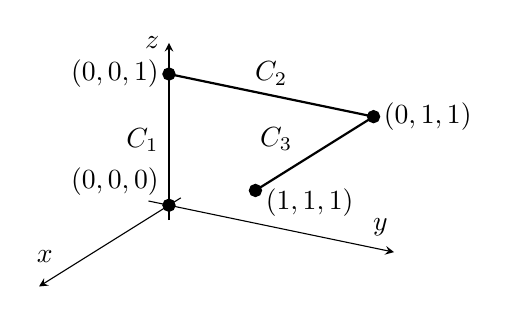
\begin{tikzpicture}[]
\begin{axis}[clip=false,small,view/h=120,axis lines=middle,xlabel={$x$},ylabel={$y$},zlabel={$z$},xtick={\empty},ytick={\empty},ztick={\empty},enlargelimits=true,zlabel style={anchor=east},zmax=1.125]
\addplot3[thick,mark=*]plot coordinates {(0,0,0)(0,0,1)}node[pos=0.5,left]{$C_1$}node[pos=0,above left]{$(0,0,0)$}node[pos=1,left]{$(0,0,1)$};
\addplot3[thick]plot coordinates {(0,0,1)(0,1,1)}node[pos=0.5,above]{$C_2$}node[right]{$(0,1,1)$};
\addplot3[thick,mark=*]plot coordinates {(0,1,1)(1,1,1)}node[pos=0.6,above left]{$C_3$}node[right,yshift=-1ex]{$(1,1,1)$};
\end{axis}
\end{tikzpicture}
\caption{ٹکڑوں میں خطی راہ برائے سوال \حوالہ{سوال_سمتی_تکمل_ٹکڑوں_خطی_راہ}}
\label{شکل_سوال_سمتی_تکمل_ٹکڑوں_خطی_راہ}
\end{minipage}
\end{figure}
\ابتدا{سوال}\شناخت{سوال_سمتی_تکمل_دائری_راہ}
تفاعل \عددی{f(x,y,z)=x+\sqrt{y}-z^2} کا تکمل \عددی{(0,0,0)} تا \عددی{(1,1,1)} درج ذیل راہ پر  چلتے ہوئے  تلاش کریں  (شکل \حوالہ{شکل_سوال_سمتی_تکمل_دائری_راہ})۔
\begin{align*}
C_1:\quad \kvec{r}(t)&=t\ai+t^2\aj,\quad 0\le t\le 1\\
C_2:\quad \kvec{r}(t)&=\ai+\aj+t\ak,\quad 0\le t\le 1
\end{align*}
\انتہا{سوال}
%
\ابتدا{سوال}\شناخت{سوال_سمتی_تکمل_ٹکڑوں_خطی_راہ}
تفاعل \عددی{f(x,y,z)=x+\sqrt{y}-z^2} کا تکمل \عددی{(0,0,0)} تا \عددی{(1,1,1)} درج ذیل راہ پر  چلتے ہوئے  تلاش کریں  (شکل \حوالہ{شکل_سوال_سمتی_تکمل_ٹکڑوں_خطی_راہ})۔
\begin{align*}
C_1:\quad \kvec{r}(t)&=t\ak,\quad 0\le t\le 1\\
C_2:\quad \kvec{r}(t)&=t\aj+\ak,\quad 0\le t\le 1\\
C_3:\quad \kvec{r}(t)&=t\ai+\aj+\ak,\quad 0\le t\le 1
\end{align*}

\انتہا{سوال}
%
\ابتدا{سوال}
تفاعل \عددی{f(x,y,z)=\tfrac{x+y+z}{x^2+y^2+z^2}} کا تکمل راہ \عددی{\kvec{r}(t)=t\ai+t\aj+t\ak,\, 0<a\le t\le b} پر تلاش کریں۔
\انتہا{سوال}
%
\ابتدا{سوال}
تفاعل \عددی{f(x,y,z)=-\sqrt{x^2+z^2}} کا تکمل درج ذیل دائری راہ پر تلاش کریں۔
\[\kvec{r}(t)=(a\cos t)\ai+(a\sin t)\ak,\quad 0\le t\le 2\pi\]
\انتہا{سوال}
%
\موٹا{مسطح منحنیات پر لکیری تکملات}\\
سوال \حوالہ{سوال_سمتی_تکمل_دی_گئی_منحنی-الف} تا سوال \حوالہ{سوال_سمتی_تکمل_دی_گئی_منحنی-ب} میں \عددی{f} کا تکمل دی گئی منحنی پر تلاش کریں۔

\ابتدا{سوال}\شناخت{سوال_سمتی_تکمل_دی_گئی_منحنی-الف}
\(f(x,y)=\frac{x^3}{y},\quad C:\, y=\frac{x^2}{2},\quad 0\le x\le 2\)
\انتہا{سوال}
%
\ابتدا{سوال}
\(f(x,y)=\frac{x+y^2}{\sqrt{1+x^2}},\quad C:\, y=\frac{x^2}{2},\quad \text{\RL{ \عددی{(1,\frac{1}{2})} سے \عددی{(0,0)} تک}}\)
\انتہا{سوال}
%
\ابتدا{سوال}
\(f(x,y)=x+y,\quad C:\, x^2+y^2=4,\quad \text{\RL{  ربع اول میں \عددی{(2,0)} سے \عددی{(0,2)} تک}}\)
\انتہا{سوال}
%
\ابتدا{سوال}\شناخت{سوال_سمتی_تکمل_دی_گئی_منحنی-ب}
\(f(x,y)=x^2-y,\quad C:\, x^2+y^2=4,\quad \text{\RL{  ربع اول میں \عددی{(0,2)} سے \عددی{(\sqrt{2},\sqrt{2})} تک}}\)
\انتہا{سوال}

\موٹا{کمیت اور معیار اثر}\\
%
\ابتدا{سوال}
ایک پتلی تار جس کی کثافت \عددی{\delta=\tfrac{3}{2}t} ہے منحنی \عددی{\kvec{r}(t)=(t^2-1)\aj+2t\ak,\, 0\le t\le 1} کے ساتھ ساتھ پائی جاتی ہے۔اس تار کی کمیت تلاش کریں۔
\انتہا{سوال}
%
\ابتدا{سوال}
ایک پتلی  تار جس کی کثافت \عددی{\delta(x,y,z)=15\sqrt{y+2}} ہے منحنی \عددی{\kvec{r}(t)=(t^2-1)\aj+2t\ak,\, -1\le t\le 1} کے ساتھ ساتھ پائی جاتی ہے۔اس تار کا مرکز کمیت تلاش کریں۔ اس منحنی کو ترسیم کر کے اس پر مرکز کمیت دکھائیں۔
\انتہا{سوال}
%
\ابتدا{سوال}
منحنی \عددی{\kvec{r}(t)=\sqrt{2}t\aj+(4-t^2)\ak\, 0\le t\le 1} کے ساتھ ساتھ  ایک پتلی تار پائی جانے والی تار کی کثافت (ا) \عددی{\delta=3t}، (ب) \عددی{\delta=1} ہے۔اس تار کا مرکز کمیت تلاش کریں۔
\انتہا{سوال}
%
\ابتدا{سوال}
ایک پتلی تار جس کی کثافت \عددی{\delta=3\sqrt{5+t}} ہے منحنی
 \عددی{\kvec{r}(t)=t\ai+2t\aj+\tfrac{2}{3}t^{3/2}\ak,\, 0\le t\le 2} کے ساتھ ساتھ پائی جاتی ہے۔ اس تار کی کمیت تلاش کریں۔
\انتہا{سوال}
%
\ابتدا{سوال}
مستوی \عددی{xy} میں دائرہ \عددی{x^2+y^2=a^2} پر مستقل کثافت \عددی{\delta} کی ایک پتلی تار پائی جاتی ہے۔ محور \عددی{z} کے لحاظ سے اس تار کا جمودی معیار اثر اور رداس  دوار تلاش کریں۔
\انتہا{سوال}
%
\ابتدا{سوال}
مستوی \عددی{yz} میں لکیری قطع \عددی{\kvec{r}(t)=t\aj+(2-2t)\ak,\, 0\le t\le 1} پر مستقل کثافت  کی ایک پتلی تار پائی جاتی ہے۔ تینوں محددی محوروں  کے لحاظ سے اس تار کا جمودی معیار اثر اور رداس  دوار تلاش کریں۔
\انتہا{سوال}
%
\ابتدا{سوال}
مستقل کثافت \عددی{\delta} کی ایک پتلی تار پیچدار منحنی \عددی{\kvec{r}(t)=(\cos t)\ai+(\sin t)\aj+t\ak,\, 0\le t\le 2\pi} کے ساتھ ساتھ پائی جاتی ہے۔ (ا) \عددی{I_z} اور \عددی{R_z} تلاش کریں۔ (ب) فرض کریں مستقل کثافت \عددی{\delta} کی ایک دوسری پتلی تار، جس کی لمبائی دگنی ہے (\عددی{0\le t\le 4\pi})، اسی منحنی \عددی{\kvec{r}(t)} کے ساتھ ساتھ پائی جاتی ہے۔ بغیر حل کیے بتلائیں کہ آیا اس تار کا جمودی معیار اثر اور رداس دوار پہلی تار سے مختلف ہوں گے؟  اب انہیں حل کر کے اپنے جواب کی تصدیق کریں۔
\انتہا{سوال}
%
\ابتدا{سوال}
منحنی \عددی{\kvec{r}(t)=(t\cos t)\ai+(t\sin t)\aj+(\tfrac{2\sqrt{2}}{3})t^{3/2}\ak,\, 0\le t\le 1} کے ساتھ ساتھ مستقل کثافت \عددی{\delta =1} کی ایک پتلی تار  پائی جاتی ہے۔ اس کی \عددی{\overline{z}}، \عددی{I_z} اور \عددی{R_z} تلاش کریں۔
\انتہا{سوال}
%
\ابتدا{سوال}
\عددی{I_z} اور \عددی{R_z} مثال \حوالہ{مثال_سمتی_تکمل_قوس_کی_کمیت} کی محراب کے لئے تلاش کریں۔
\انتہا{سوال}
%
\ابتدا{سوال}
ایک پتلی تار جس کی کثافت \عددی{\delta=\tfrac{1}{t+1}} ہے منحنی \عددی{\kvec{r}(t)=t\ai+\tfrac{2\sqrt{2}}{3}t^{3/2}\aj+\tfrac{t^2}{2}\ak,\, 0\le t\le 2} کے ساتھ ساتھ پائی جاتی ہے۔ اس تار کا مرکز کمیت اور محددی محوروں کے لحاظ سے جمودی معیار اثر اور رداس دوار تلاش کریں۔
\انتہا{سوال}
\موٹا{کمپیوٹر کا استعمال}\\
سوال \حوالہ{سوال_سمتی_تکمل_کمپیوٹر_الف} تا سوال \حوالہ{سوال_سمتی_تکمل_کمپیوٹر_ب} میں کمپیوٹر پر درج ذیل اقدام سے تکمل کی قیمت تلاش کریں۔
\begin{enumerate}[a.]
\item
راہ \عددی{\kvec{r}(t)=g(t)\ai+h(t)\aj+k(t)\ak} کے لئے \عددی{\dif s=\abs{\kvec{v}(t)}\dif t} دریافت کریں۔
\item
متکمل \عددی{f(g(t),h(t),k(t))\abs{\kvec{v}(t)}} کو مقدار معلوم \عددی{t} کا تفاعل لکھیں۔
\item
تکمل \عددی{\int_C f\dif s} کی قیمت مساوات \حوالہ{مساوات_میدان_خطی_تکمل_پ} کی مدد سے حاصل  کریں۔ 
\end{enumerate}
%
\ابتدا{سوال}\شناخت{سوال_سمتی_تکمل_کمپیوٹر_الف}
\(f(x,y,z)=\sqrt{1+30x^2+10y};\quad \kvec{r}(t)=t\ai+t^2\aj+3t^2\ak,\quad 0\le t\le 2\)
\انتہا{سوال}
%
\ابتدا{سوال}
\(f(x,y,z)=\sqrt{1+x^3+5y^3};\quad \kvec{r}(t)=t\ai+\frac{1}{3}t^2\aj+\sqrt{t}\ak,\quad 0\le t\le 2\)
\انتہا{سوال}
%
\ابتدا{سوال}
\(f(x,y,z)=x\sqrt{y}-3z^2;\,\kvec{r}(t)=\cos 2t \ai+\sin 2t\aj+5t\ak,\quad 0\le t\le 2\pi\)
\انتہا{سوال}
%
\ابتدا{سوال}\شناخت{سوال_سمتی_تکمل_کمپیوٹر_ب}
\(f(x,y,z)=\big(1+\frac{9}{4}z^{1/3}\big)^{1/4};\, \kvec{r}(t)=\kvec{r}(t)=\cos 2t \ai+\sin 2t\aj+t^{5/2}\ak,\)\\
\( 0\le t\le 2\pi\quad\quad\quad\quad\quad\quad\)
\انتہا{سوال}
\انتہا{سوالات}
